\newpage
\section{Source Code}
Wazuh source code is publicly available on github. There are 24 public repositories associated with Wazuh, each containing modules for the core back-end, search index, front-end, documentation etc. 

\subsection{Repositories}
Below are the four primary repositories associated with the Wazuh project:

\paragraph*{Wazuh}
\begin{description}
    \item[Repository URL:] \url{https://github.com/wazuh/wazuh}
    \item[Description:] This repository contains the backend source code for Wazuh Managers and Agents written in C, C++ and Python.
\end{description}

\paragraph*{Wazuh Dashboard}
\begin{description}
    \item[Repository URL:] \url{https://github.com/wazuh/wazuh-dashboard}
    \item[Description:] Wazuh dashboard is a fork of the OpenSearch Dashboards which incorporate changes to make it easier to use for Wazuh users. It doesn't provide any specific UI, rather it is the platform on which Wazuh web UI runs on.
\end{description}

\paragraph*{Wazuh Dashboard Plugins}
\begin{description}
    \item[Repository URL:] \url{https://github.com/wazuh/wazuh-dashboard-plugins}
    \item[Description:] This repository contains a set of plugins for Wazuh dashboard. Essentially providing all the UI components used on the Wazuh Web app.
\end{description}

\paragraph*{Wazuh Indexer}
\begin{description}
    \item[Repository URL:] \url{https://github.com/wazuh/wazuh-dashboard}
    \item[Description:] This repository contains a highly scalable, full-text search and analytics engine. This Wazuh central component indexes and stores alerts generated by the Wazuh server and provides near real-time data search and analytics capabilities.
\end{description}

\subsection{Overview of the Core Wazuh Source Code}
This section offers a high-level overview of the \href{https://github.com/wazuh/wazuh}{codebase}. Each section of the codebase is discussed briefly below:

\begin{itemize}
    \item \textbf{Architecture:} The \texttt{wazuh-db} folder contains a daemon responsible for managing access to SQLite database files. It handles automatic database upgrades, serialized and parallel queries, and other database-related tasks. Additionally, the \texttt{Metrics} folder contains metrics aiding in understanding the behavior of Wazuh components. The \texttt{syscollector} folder implements modules named Syscollector, Data Provider, DBSync, and RSync, responsible for collecting system information such as processes, hardware details, packages, OS specifics, network, and ports.
    
    \item \textbf{API:} This section includes code handling all Wazuh APIs and Wazuh API installer functions.
    
    \item \textbf{Active-response:} Here, active response scripts are managed, including default Wazuh scripts like \texttt{restart-wazuh}, \texttt{host-deny}, and \texttt{disable-account}.
    
    \item \textbf{addagent:} This section involves code related to managing Wazuh agents, including key management and server connections.
    
    \item \textbf{agentlessd:} It deals with agentless entry into hosts via SSH connections.
    
    \item \textbf{analysisd:} Crucial for analyzing events and collected logs, this section contains default decoders, pre-decoders, and rules for matching events. It also manages event creation and storage for dashboard display. The \texttt{alerts} folder stores different kinds of alerts seen in the security event section of the dashboard. It encompasses three important steps: pre-decoding, decoding, and rule-matching. All codes for default decoders and pre-decoders are present in this folder and its internal subfolders. The \texttt{compiled-rules} subfolder contains all the rules to be matched and relevant codes. Moreover, this section analyzes events and creates and stores new events to show on the dashboard.
    
    \item \textbf{agent-client:} Responsible for managing the state of agents in client endpoints, including client restarts and forwarding security events.
    
    \item \textbf{error\_messages:} This section contains header files with various error messages used across Wazuh components.
    
    \item \textbf{headers:} Comprising miscellaneous headers and utility functions, it includes functionalities ranging from cryptography to file queues.
    
    \item \textbf{init:} Handles new user and group creation, deletion, and agent registration to servers.
    
    \item \textbf{logcollector:} Manages log data collection via agents or direct transmission to the server using the rsyslog protocol.
    
    \item \textbf{monitord:} Monitors logs and generates reports based on log data.
    
    \item \textbf{remoted:} Implements remote communication functionalities like sending messages, handling the syslog protocol, and facilitating shared downloads.
    
    \item \textbf{reportd:} Generates reports based on various input parameters.
    
    \item \textbf{Rootcheck:} Allows defining policies to check if agents meet specified requirements, including process checks, file presence, and content patterns. This feature is implemented in this section.
    
    \item \textbf{utils:} Contains helper functions and code related to agent control, agent listing, and verifying agent configurations. It also houses switch-cases for navigation from the command line.
    
    \item \textbf{wazuh\_db:} Contains schema definitions for different Wazuh databases, including those for agents, modules (covered later), upgrades (all versions), rootcheck, etc.
    
    \item \textbf{wazuh\_modules:} Houses main modules such as agent upgrade, syscollector (gathering system information), and task manager (coordinating and scheduling tasks between manager and agents).
    
    \item \textbf{syscheck:} Manages system integrity checking, including verifying file integrity and detecting system changes.
    
    \item \textbf{filebeat:} Integrates Filebeat with Wazuh, enabling log collection and analysis.
\end{itemize}

\subsection{Compiling the Front-end from Source}
From the repository structure and descriptions, it was evident that \texttt{wazuh-dashboard-plugins} repository hosted all of the front-end source code.

We followed the contributor's guide and documentation to compile the repository and create a development environment for the front-end. The steps to recreate the environment is outlined below-

\begin{enumerate}
    \item Remove or disable standalone Docker Engine (if installed). Install \href{https://docs.docker.com/get-docker/}{Docker Desktop}.
    \item Configure the docker environment.
    \begin{minted}{bash}
docker network create devel
docker network create mon
docker plugin install grafana/loki-docker-driver:latest \
    --alias loki --grant-all-permissions
    \end{minted}
    \item Assign enough resources to Docker Desktop. At least -
    \begin{itemize}
        \item 8 GB of RAM
        \item 4 CPU Cores
    \end{itemize}
    \item Save the path to the \texttt{plugins} folder inside \texttt{wazuh-dashboard-plugins} repository code as an environment variable, by exporting this path on .bashrc, .zhsrc or similar.
    \begin{minted}{bash}
./bashrc
export WZ_HOME=~/code/wazuh-dashboard-plugins/plugins
    \end{minted}
    \item The Docker volumes will be created by the internal Docker user, making them read-only. Which will prevent us from modifying the source code while running the environment. To prevent this, a new group named \texttt{docker-desktop} and GUID 100999 needs to be created, then added to the user and the source code folder:
    \begin{minted}{bash}
sudo groupadd -g 100999 docker-desktop
sudo useradd -u 100999 -g 100999 -M docker-desktop
sudo chown -R $USER:docker-desktop $WZ_HOME
sudo chmod -R 774 $WZ_HOME
sudo usermod -aG docker-desktop $USER
    \end{minted}
    \item Clone the repository.
    \begin{minted}{bash}
git clone https://github.com/wazuh/wazuh-dashboard-plugins.git
cd wazuh-dashboard-plugins
    \end{minted}
    \item Checkout to tag \texttt{v4.7.2-2.8.0}, corresponding to \texttt{Wazuh v4.7.2} release with \texttt{OpenSearch Dashboards 2.8.0}.
    \begin{minted}{bash}
git checkout v4.7.2-2.8.0
    \end{minted}

    \item The \texttt{docker} folder inside the repository contains various docker images to create development and testing environments. We use the \texttt{osd-dev} environment.
    \begin{minted}{bash}
cd docker/osd-dev
    \end{minted}
    \item Use the \texttt{dev.sh} script to call \texttt{docker-compose} and spin up the containers required for the development environment.
    \begin{minted}{bash}
./dev.sh 2.8.0 2.8.0 $WZ_HOME/main up server 4.7.2
    \end{minted}
    where, 
    \begin{itemize}
        \item \texttt{os\_version=2.8.0} is the OpenSearch version
        \item \texttt{osd\_version=2.8.0} is the OpenSearch Dashboard version
        \item \texttt{os\_version=\$WZ\_HOME/main} is the path to the Wazuh Application source code
        \item \texttt{action=up} is the action to do (one of \texttt{up}, \texttt{down} or \texttt{stop}.
        \item \texttt{server} to create an environment with a Wazuh Server running.
        \item \texttt{server\_version} version of the Wazuh server.
    \end{itemize}
    \item Also, add a agent container with the command:
    \begin{minted}{bash}
docker run --name os-dev-280-agent-$(date +%s) \
    --network os-dev-2.8.0 \
    --label com.docker.compose.project=os-dev-280 \
    --env WAZUH_AGENT_VERSION=4.7.2 \
    -d ubuntu:20.04 bash -c 
    'apt update -y
    apt install -y curl lsb-release
    curl -so \wazuh-agent-${WAZUH_AGENT_VERSION}.deb \
        "https://packages.wazuh.com/4.x/apt/pool/main/w/wazuh-agent/"\
        "wazuh-agent_${WAZUH_AGENT_VERSION}-1_amd64.deb" \
        && WAZUH_MANAGER='wazuh.manager' WAZUH_AGENT_GROUP='default' \
        dpkg -i ./wazuh-agent-${WAZUH_AGENT_VERSION}.deb
    /etc/init.d/wazuh-agent start
    tail -f /var/ossec/logs/ossec.log'
    \end{minted}
    \item Attach a shell to the \texttt{os-dev-280-osd-1} docker container to go inside the development environment.
    \begin{minted}{bash}
docker exec -it os-dev-280-osd-1 /bin/bash
    \end{minted}
    \item Install the dependencies using:
    \begin{minted}{bash}
yarn install 
    \end{minted}
    \item Run the Web server on \texttt{https://0.0.0.0:5601/} using:
    \begin{minted}{bash}
yarn start --no-base-path 
    \end{minted}
\end{enumerate}
The server usually takes a few moments to load all the comments. Once it's loaded login using credentials \texttt{admin:admin}.

As a demonstration, we place a new name in the dashboard title bar.
    \begin{figure} [H]
        \centering
        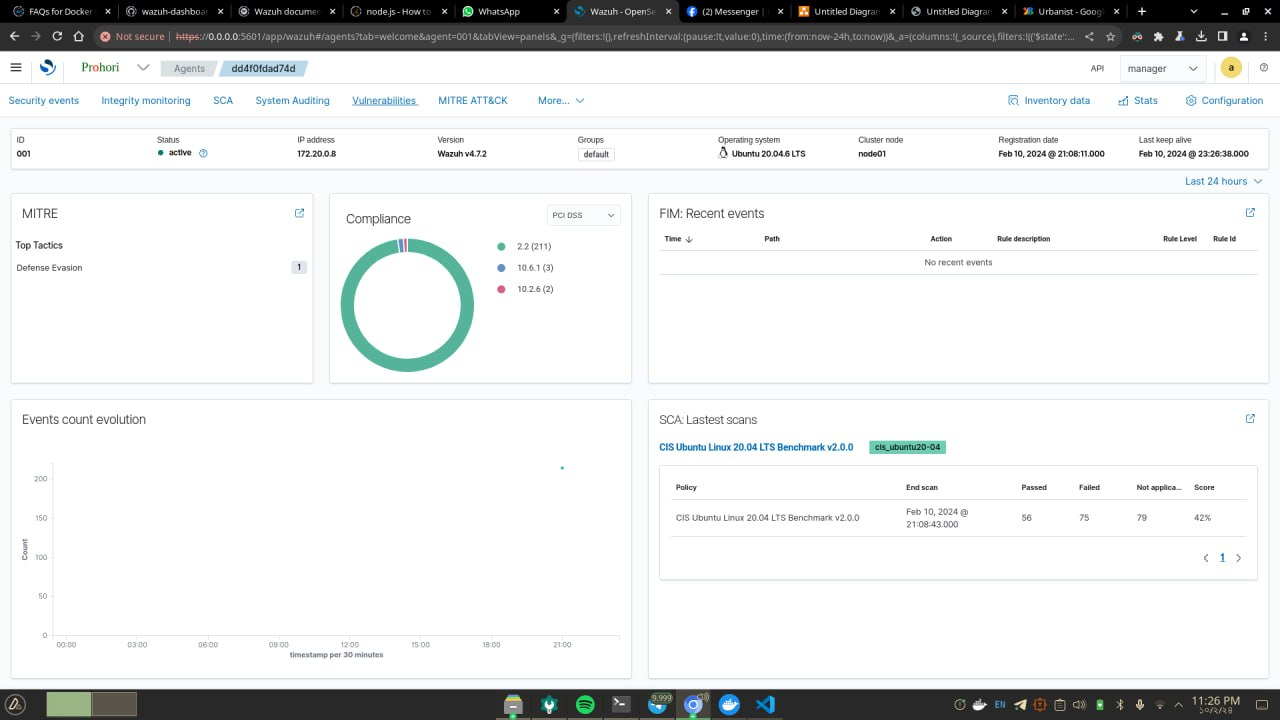
\includegraphics[width=0.9\textwidth]{images/prohori.jpg}
        \caption{Wazuh Dashboard with Custom Title - Prohori}
        \label{fig:prohori}
    \end{figure}
Needless to say, getting this done opens a door of endless possibilities for us to customize the dashboard and add new features to it. Even more importantly, there is a commercial aspect to it. We can now offer our services to other organizations to customize their Wazuh dashboards as per their requirements.